
\documentclass[12]{article}
\usepackage[utf8]{inputenc}
\usepackage{cite}

\author{par4111 \\ Adrià Cabeza, Xavier Lacasa \\ Departament d' Arquitectura de Computadors}
\title{Lab 4: Divide and Conquer parallelism with OpenMP: Sorting }
\date{\today \\ 2018 - 19 SPRING}
\usepackage{graphicx}
%\usepackage[left=3.5cm, right=3.5cm]{geometry}
\usepackage{subcaption}
\usepackage{pgfplots}
\usepackage{listings}
\usepackage[margin=1.25in]{geometry}
\usepackage{xcolor}
\usepackage{float}
\lstset{
  basicstyle=\ttfamily,
  showstringspaces=false,
  commentstyle=\color{purple},
  keywordstyle=\color{blue},
	frame=tb,language=python,breaklines=true,numbers=none,  stringstyle=\color{red}, tabsize=3,   showstringspaces=false,
  columns=flexible, 
}
\begin{document}
\maketitle

\vspace*{\fill}
\begin{center}

\includegraphics[scale=0.35]{images/UPClogo.png}
\end{center}
\newpage
\tableofcontents
\newpage
\section{Introduction}
In this laboratory session we are going to practice and observe different parallelization strategies on a recursive algorithm : \textbf{Multisort}.

This algorithm can be spitted in a lot of little different tasks with smaller problem size and then merged into one (following the divide and conquer strategy).
\\
To begin we will start by analyzing the parallelism of \textbf{multisort-tareador.c} code provided in order to fully understand its dependencies and develop a proper parallelized version of it.
\\
Then, three different parallelization strategies will we considered: \textbf{Leaf} strategy, \textbf{Tree} strategy and \textbf{Tree} strategy using a \textbf{cut-off} mechanism based on recursion level. 
\\
Finally TODO 


\section{Analysis with Tareador}
The multisort algorithm is composed by two functions: the merge function and the multisort function itself.
In the mulisort function, recursive decomposition is done by dividing the data vector into four parts and each of these parts into four parts, until we reach leafs (base case), where we call the \textit{basicsort} function.  During the recursive decomposition, we also merge the sorted parts two by two. 


\subsection{Merge Function}
For the merge function, in order to see the potentially parallelizable parts of the code, we created a task for each recursive call to the merge function. With this approach a task is generated for each of the nodes of the merge recursion tree, and the children (in this case the merge functions that call \textit{basic merge}) are going to be executed for the same task that calls \textit{basic merge}. 
\\
\medskip
\begin{lstlisting}[frame=single]
void merge(long n, T left[n], T right[n], T result[n*2], long start, long length) {
        if (length < MIN_MERGE_SIZE*2L) {
                // Base case
                basicmerge(n, left, right, result, start, length);
        } else {
                // Recursive decomposition
               tareador_start_task("Forth merge");
                 merge(n, left, right, result, start, length/2);
                tareador_end_task("Forth merge");
                tareador_start_task("Fifth merge");
                merge(n, left, right, result, start + length/2, length/2);
                tareador_end_task("Fifth merge");
         }
}
\end{lstlisting}
\subsection{Multisort Function}
For the multisort function the same strategy as in the merge function is selected. In order to generate the maximum parallelism (and then study the task dependencies) a task is created for each call to the multisort and merge functions. A task creation is not needed in the \textit{basicsort} function because the multisort task that calls to this function can execute the code of the function. 
\\
\medskip

\begin{lstlisting}[frame=single]
void multisort(long n, T data[n], T tmp[n]) {
        if (n >= MIN_SORT_SIZE*4L) {
                // Recursive decomposition
                tareador_start_task("First multisort");
                multisort(n/4L, &data[0], &tmp[0]);
                tareador_end_task("First multisort");
                tareador_start_task("Second multisort");
                multisort(n/4L, &data[n/4L], &tmp[n/4L]);
                tareador_end_task("Second multisort");
                tareador_start_task("Third multisort");
                multisort(n/4L, &data[n/2L], &tmp[n/2L]);
                tareador_end_task("Third multisort");
                tareador_start_task("Forth multisort");
                multisort(n/4L, &data[3L*n/4L], &tmp[3L*n/4L]);
                tareador_end_task("Forth multisort");
                tareador_start_task("First merge");
                merge(n/4L, &data[0], &data[n/4L], &tmp[0], 0, n/2L);
                tareador_end_task("First merge");
                tareador_start_task("Second merge");
                merge(n/4L, &data[n/2L], &data[3L*n/4L], &tmp[n/2L], 0, n/2L);
                tareador_end_task("Second merge");
                tareador_start_task("Third merge");
                merge(n/2L, &tmp[0], &tmp[n/2L], &data[0], 0, n);
                tareador_end_task("Third merge");

        } else {
                // Base case
                basicsort(n, data);
        }
}

\end{lstlisting}


\subsection{Task dependency graph}

In Figure \ref{multisort_paraver} you can observe the task dependency graph. The first 2 layers (beginning from the top) show the list being divided into 4 parts and each part into 4 more to be sorted, so 16 parts in total (these sort calls tasks are represented by the green circles, red trapezes, yellow squares and pink octagons which appear twice each, hence the so called 2 layers).  Then, each 2 contiguous parts are merged together, which is why the previous shapes point to a smaller dot which is the same for every 2 shapes. It means that merging 2 parts has a dependency which is each part being sorted. This merge calls itself 2 times (which create the red octagon and green parallelogram). Now these 2 merged parts are merged with 2 other merged parts, and it appears that merge now calls itself 2 times and each calls itself another 2 times, which then execute basicmerge, that when completed result in the 2 parts being merged. Here ends the part represented by the first layer of "big semi-transparent squares which contain tasks" in Figure \ref{multisort_paraver}. At this point the 16 originals parts of the layer 2  have been sorted and merged into the big 4 parts of the layer 1, meaning now we have the list divided into 4 parts, each sorted. Now a merge for each 2 tasks occur, which in turn calls 2 merges and each of these call 2 merges again, which execute basicmerge, this explains the middle "big semi-transparent squares". And finally, with only the 2 halves of the list to put together, merge is called again, and this time calls itself in a recursion of 4 levels, resulting in the bottom row of "big semi-transparent squares" of Figure \ref{multisort_paraver}, which end in one single dot which is the task where the whole list is finally sorted.

\begin{figure}[H]
    \centering
    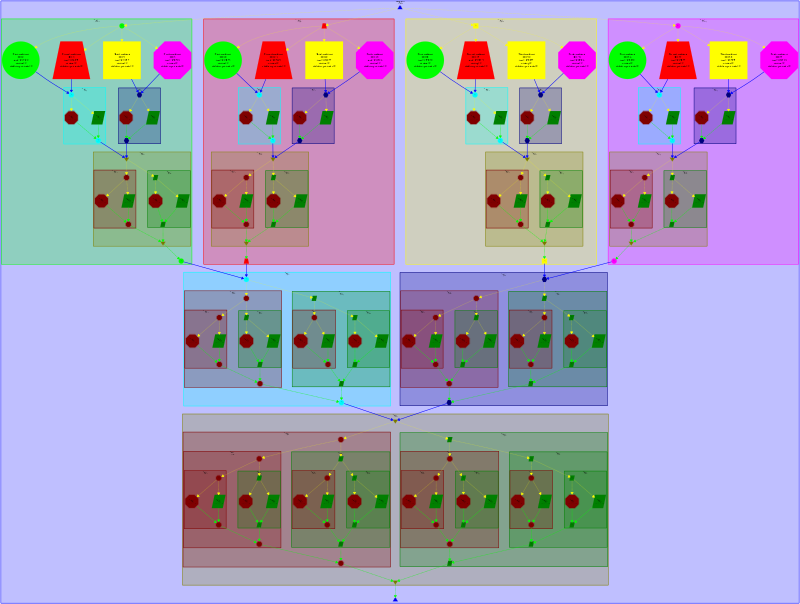
\includegraphics[scale=0.40]{images/multisort_tareador.png}
    \caption{Multisort algorithm task dependence graph}
    \label{multisort_paraver}
\end{figure}

\subsection{Execution Time and Speed-up for different \#Threads}

\begin{center}
\begin{tabular}{|c|c|c|}
 \hline 
   \textbf{Threads} & \textbf{Execution Time ($ \mu$s)} & \textbf{Speed-up} \\  \hline
     1 & 20.334.411 & 1.0000\\ \hline
     2 & 10.173.716 & 1.9987\\  \hline
     4 & 5.086.725 & 3.9975\\  \hline
     8 & 2.550.595 & 7.9724 \\  \hline
     16 & 1.289.922 & 15.7640 \\  \hline
     32 & 1.289.909 & 15.7642\\  \hline
     64 & 1.289.909 & 15.7642\\  \hline
                                
\end{tabular}
\end{center}
\begin{figure}[H]
    \centering
    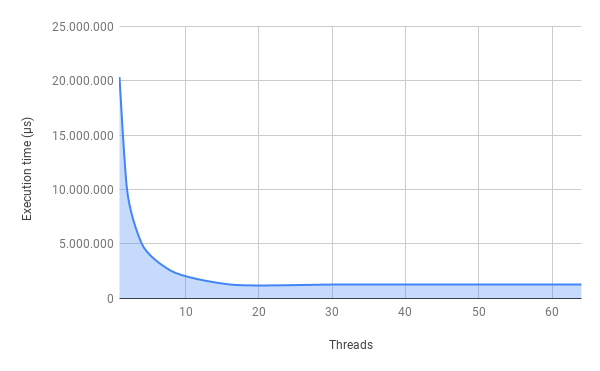
\includegraphics[scale=0.60]{images/chart0.png}
    \caption{Execution time plot}
    \label{chart0}
\end{figure}
\begin{figure}[H]
    \centering
    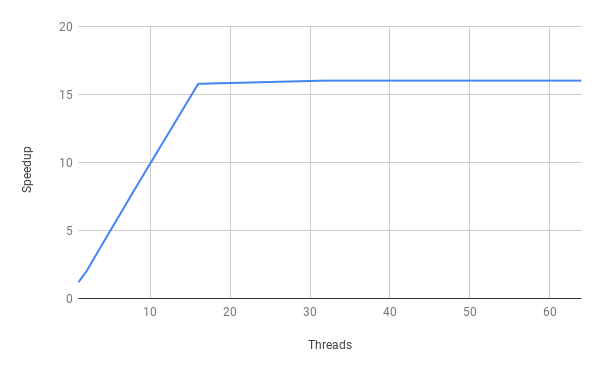
\includegraphics[scale=0.60]{images/chart1.png}
    \caption{Speed-up plot}
    \label{chart1}
\end{figure}


We can see that, from 1 to 16 processors, when we double the amount of processors we obtained a nice Speed-up, around 2. However, when we use more than 16 processors we do not see an increment in the Speed-up because there is no much work left to do for the rest of the processors so they are useless. Moreover, the Speed-up we get from 1 to 16 processors is \textbf{pretty close to the ideal one}. As we keep doubling the number of processors, Speed-up keeps roughly doubling.

\section{Parallelization and performance analysis with tasks}
As we mentioned before, we have two options whenever we have to parallelize code: \textit{Leaf strategy}, which consists in creating a task for each leaf in the dependency graph (with the additional task doing all the recursion and generating the tasks) and a \textit{Tree Strategy}, which consists in creating a task for each node in the tree. 


\subsection{Leaf Strategy}
This strategy consists in creating a task for each leaf in the tree generated by making the recursive calls. 
\\
In order to accomplish this strategy, we have placed a \textbf{\#pragma omp task} before each terminating function (any function inside merge and multisort that does not have recursion: basicmerge and basicsort). Also, we need a way to synchronize different tasks in order to avoid data races and fulfill the data dependencies. We have done it inserting \textbf{taskgroup} directives.
\\
\medskip

\begin{lstlisting}[frame=single]
void merge(logn n, T left[n], T right[n], T result[n*2], long start, long length){
if (length < MIN_MERGE_SIZE*2L){
    //BASE case
    #pragma omp task
    basicmerge(n,left,right,result,start,length);
} else {
    //Recursive decomposition
    merge(n,left,right,result,start,length/2);
    merge(n,left,right,result,start+length/2, length/2);
    }
}

void multisort(long n, T data[n], T tmp[n]){
    if(n>= MIN_SORT_SIZE*4L){
        // Recursive decomposition
        #pragma omp taskgroup
        {
            multisort(n/4L, &data[0], &tmp[0]);
            multisort(n/4L, &data[n/4L], &tmp[n/4L]);
            multisort(n/4L, &data[n/2L], &tmp[n/2L]);
            multisort(n/4L, &data[3L*n/4L], &tmp[3L*n/4L]);
        }
        
        #pragma omp taskgroup
        {
            merge(n/4L, &data[0], &data[n/4L], &tmp[0],0,n/2L);
            merge(n/4L, &data[n/2L], &data[3L*n/4L], &tmp[n/2L],0,n/2L);
        }
        
        merge(n/2L, &tmp[0], &tmp[n/2L], &data[0], 0, n);
    } else{
            //Base case
            #pragma omp task
            basicsort(n,data);
    }
}

int main(...) {
    ...
    #pragma omp parallel
    #pragma omp single
    multisort(N, data, tmp);
    ...
}
\end{lstlisting}
\medskip

In this strategy we have one thread that generates all the tasks, and then a thread executing one task for each leaf. If we analyze this strategy, we can see that parallel tasks are being created only when reaching the leaves of the recursion, which results in having many sequential fragments all the way through the 'recursion path'. Because of this, speed-up isn't as good as it could be. The following Paraver captures in Figure \ref{paraverleaf} and \ref{paraverleafZoom} show this in more detail (Note the traces have been generated in Boada 1 because we couldn't execute it anywhere else due to a missing file error of mpi2prv). For all Paraver traces, we will display at the top the standard configuration, and below it the Task configuration, which will let us appreciate when a task is created and when it is executed.
\\
\medskip
\begin{figure}[H]
    \centering
    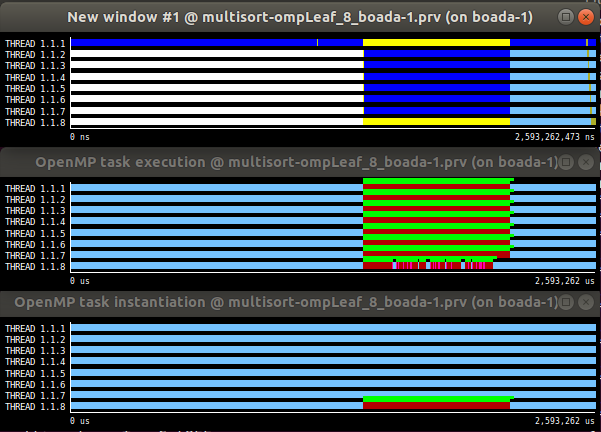
\includegraphics[scale=0.75]{images/paraverLeafNoZoom.PNG}
    \caption{Paraver with a Leaf strategy}
    \label{paraverleaf}
\end{figure}
In Figure \ref{paraverleaf} it is clear how Thread 8 goes through all the recursion until reaching the leaves, which is when it starts creating tasks and other threads start executing them. This is why task generation is so delayed.

\medskip
\begin{figure}[H]
    \centering
    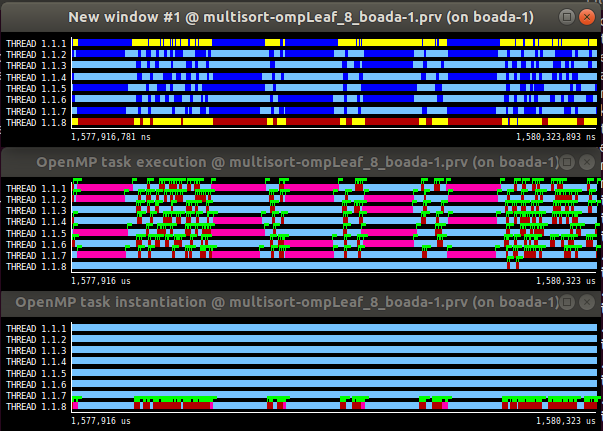
\includegraphics[scale=0.75]{images/paraverLeafZoom.PNG}
    \caption{Paraver with a Leaf strategy, zoomed in}
    \label{paraverleafZoom}
\end{figure}

In Figure \ref{paraverleafZoom} we can see more clearly what's happening during task creation. We can appreciate how merge (pink) seems to take way a longer time to complete than quicksort (red). In fact, what explains why this strategy can't take advantage of all 8 threads is that at any given time, there are only 4 threads either sorting or merging, as seen in the zoomed in trace. This happens because the list is divided into 4 parts to sort and later merge, but since they have dependencies (cannot merge the 4 parts before sorting them), no more than 4 threads can be executing tasks at any given time
\\
Checking the following plots we can see that the maximum speed-up reached is gotten with 4 threads, which was predictable given the explanation given just before (no more than 4 tasks can be executed at a time). From 4 threads on, speed-up decreases, which might be due to overhead being added by the creation of threads.
\medskip
\begin{figure}[H]
    \centering
    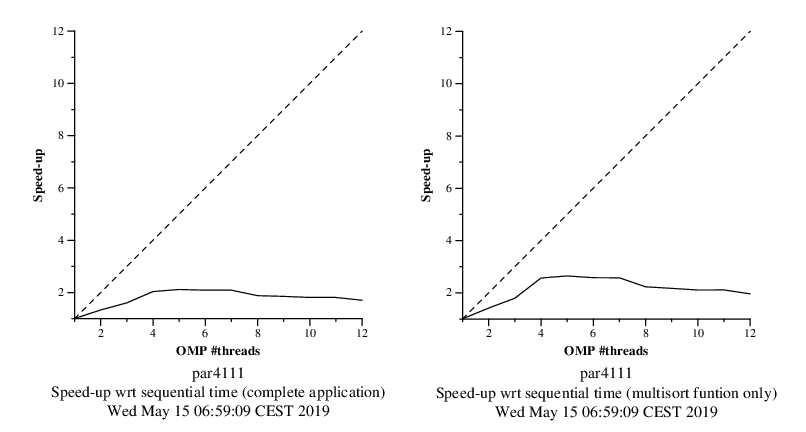
\includegraphics[scale=0.75]{images/leafStrong.png}
    \caption{Speed-up with a Leaf strategy}
    \label{speedupleaf}
\end{figure}





\subsection{Tree Strategy}
This stategy consists in creating a task for each call inside a new level of recursivity, generating parallelism and improving the speed-up of the program. 
\\
In order to accomplish this strategy, we have placed a \textbf{#pragma omp task} before each recursive call in the multisort and merge functions. Also, we need a way to synchronize the different tasks, in this case we have placed a taskgroup for the multisort calls and another taskgroup for the two first merge calls.
\\
\medskip
\begin{lstlisting}[frame=single]
void merge(long n, T left[n], T right[n], T result[n*2], long start, long length){
if (length < MIN_MERGE_SIZE*2L){
    //BASE case
    basicmerge(n,left,right,result,start,length);
} else {
    //Recursive decomposition
    #pragma omp task
    merge(n,left,right,result,start,length/2);
    #pragma omp task
    merge(n,left,right,result,start+length/2, length/2);
    }
}

void multisort(long n, T data[n], T tmp[n]){
    if(n >= MIN_SORT_SIZE*4L){
    //RECURSIVE decomposition
        #pragma omp taskgroup
        {
            #pragma omp task
            multisort(n/4L, &data[0], &tmp[0]);
            #pragma omp task
            multisort(n/4L, &data[n/4L], &tmp[n/4L]);
            #pragma omp task
            multisort(n/4L,&data[n/2L], &tmp[n/2L]);
            #pragma omp task
            multisort(n/4L,&data[3L*n/4L], &tmp[3L*n/4L]);
        }
        #pragma omp taskgroup
        {
            #pragma omp task
            merge(n/4L, &data[0], &data[n/4L], &tmp[0],0,n/2L);
            #pragma omp task
            merge(n/4L, &data[n/2L], &data[3L*n/4L], &tmp[n/2L],0,n/2L);
        }
        #pragma omp task
        merge(n/2L, &tmp[0], &tmp[n/2L],&data[0],0,n);
    }else{
    //Base case
        basicsort(n,data);    
    
    }
}

int main(...) {
    ...
    #pragma omp parallel
    #pragma omp single
    multisort(N, data, tmp);
    ...
}
\end{lstlisting}
\medskip
In this strategy we have one different thread for each call to the recursion so we are going to have more tasks and therefore more threads can work at the same time. This should give us a better speed-up than Leaf strategy, but still probably not the best, as creating a task for each recursive call will add a lot of overhead and isn't really necessary. Figure \ref{paravertree} and \ref{paravertreeZoom} show the Paraver traces of the tree strategy:
\\
\medskip
\begin{figure}[H]
    \centering
    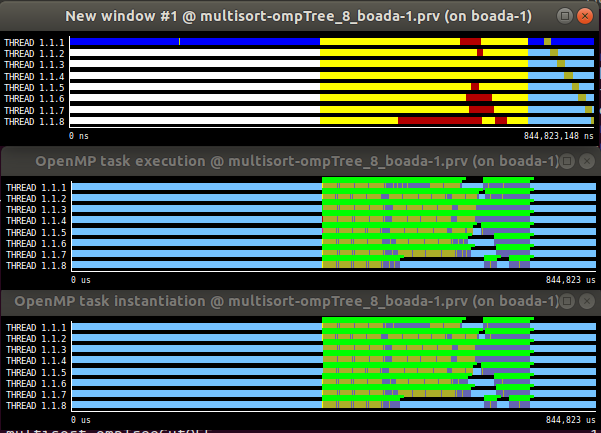
\includegraphics[scale=0.75]{images/paraverTreeNoZoom.PNG}
    \caption{Paraver with a Tree strategy}
    \label{paravertree}
\end{figure}
In Figure \ref{paravertree}, this time, it's easy to see that not only 1 thread is creating tasks, but all of them instead. The bottom configuration, which shows task instantiation, displays how all threads are busy creating tasks.

\medskip
\begin{figure}[H]
    \centering
    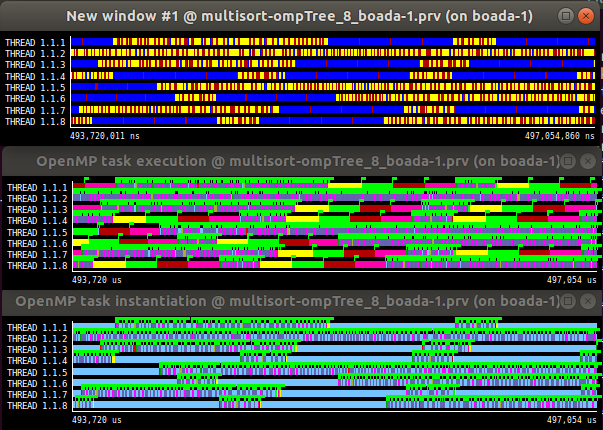
\includegraphics[scale=0.75]{images/paraverTreeZoom.PNG}
    \caption{Paraver with a Tree strategy, zoomed in}
    \label{paravertreeZoom}
\end{figure}

In Figure \ref{paravertreeZoom} we can clearly see how all threads are very busy both creating tasks and executing them. This doesn't necessarily mean it's the best strategy, as part of the reason all threads are so busy is the added overhead of creating so many tasks. We think the best strategy will probably be adding a cutoff so that at a certain recursion level task creation is stopped. This way we would gain the benefits of both a parallelized task creation strategy and reduced overhead from not fcreating so many tasks.

\\
Checking the strong scalability plots, it appears that the more threads, the better, but reaching an asymptotic end at a 3.5 speed more or less. It makes sense, as with the huge amount of tasks created, which are not dependant from one another for tasks of the same recursion level, we end up with a lot of tasks non-dependant among them near the leaves, which will take advantage of having as many threads available as possible to execute them.
\medskip
\begin{figure}[H]
    \centering
    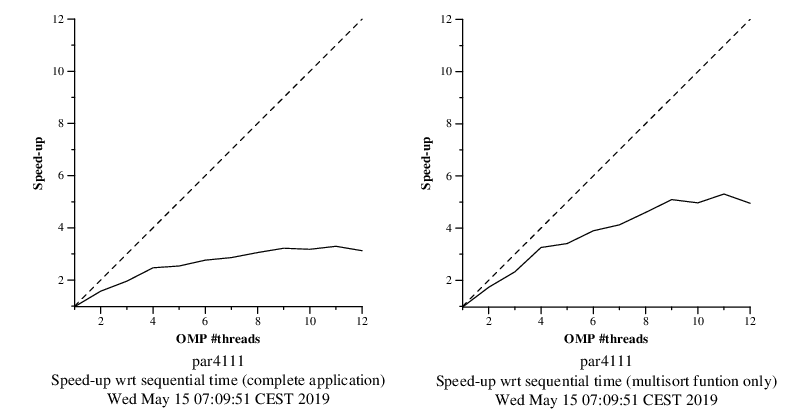
\includegraphics[scale=0.75]{images/treeStrong.png}
    \caption{Speed-up with a Tree strategy}
    \label{speeduptree}
\end{figure}

\subsection{Tree Strategy with cut-off}
\medskip

In order to improve the \textbf{Tree strategy}, we included also a cut-off mechanism based on recursion level. To implement this mechanism we have modified the code that was shown before:
\medskip

\begin{lstlisting}[frame=single]
void merge(long n, T left[n], T right[n], T result[n*2], long start, long length,int depth){
    if (length < MIN_MERGE_SIZE*2L){
        //BASE case
        basicmerge(n,left,right,result,start,length);
    } else {
        if (!omp_in_final()){
            //Recursive decomposition
            #pragma omp task final(depth >= CUTOFF)
            merge(n,left,right,result,start,length/2,depth+1);
            #pragma omp task final(depth >= CUTOFF)
            merge(n,left,right,result,start+length/2, length/2,depth+1);
        }else{
            merge(n, left, right, result, start, length/2,depth);
            merge(n,left,right, result, start+length/2,length/2,depth);
        }
    }
}

void multisort(long n, T data[n], T tmp[n],int depth){
    if(n >= MIN_SORT_SIZE*4L){
    //RECURSIVE decomposition
        if (!omp_in_final()) {
            #pragma omp taskgroup
            {
                #pragma omp task final(depth >= CUTOFF)
                multisort(n/4L, &data[0], &tmp[0],depth+1);
                #pragma omp task final(depth >= CUTOFF)
                multisort(n/4L, &data[n/4L], &tmp[n/4L],depth+1);
                #pragma omp task final(depth >= CUTOFF)
                multisort(n/4L,&data[n/2L], &tmp[n/2L],depth+1);
                #pragma omp task final(depth >= CUTOFF)
                multisort(n/4L,&data[3L*n/4L], &tmp[3L*n/4L],depth+1);
            }
            #pragma omp taskgroup
            {
                #pragma omp task final(depth >= CUTOFF)
                merge(n/4L, &data[0], &data[n/4L], &tmp[0],0,n/2L,depth+1);
                #pragma omp task final(depth >= CUTOFF)
                merge(n/4L, &data[n/2L], &data[3L*n/4L], &tmp[n/2L],0,n/2L,depth+1);
            }
            #pragma omp task final(depth >= CUTOFF)
            merge(n/2L, &tmp[0], &tmp[n/2L],&data[0],0,n,depth+1);
        } else {
                multisort(n/4L, &data[0], &tmp[0],depth);
                multisort(n/4L, &data[n/4L], &tmp[n/4L],depth);
                multisort(n/4L, &data[n/2L], &tmp[n/2L],depth);
                multisort(n/4L, &data[3L*n/4L], &tmp[3L*n/4L], depth);
                merge(n/4L, &data[0], &data[n/4L], &tmp[0],0,n/2L,depth);
                merge(n/4L, &data[0], &data[n/4L], &tmp[0],0,n/2L,depth);
                merge(n/2L, &tmp[0], &tmp[n/2L],&data[0],0,n,depth);
        }
   }else{
    //Base case
        basicsort(n,data);
    }
}

int main(...) {
    ...
    #pragma omp parallel
    #pragma omp single
    multisort(N, data, tmp, 0);
    ...
}
\end{lstlisting}
With this strategy, a tree task creation scheme is followed but, at a certain depth in the recursion, tasks stop being created meaning the rest is executed sequentially. This should be the best strategy, as mentioned earlier, because we still have a lot of parallelization due to the early levels task creation, but do not have the overhead of the tasks created in the levels near the leaves, which taking into account that the number of tasks is exponential on the depth, is a great advantage. Figure \ref{paravercutoff} and \ref{paravercutoffZoom} show the traces obtained by running multisort in a tree strategy with a cutoff depth = 0 (right at the begining of the recursion).
\\
\medskip
\begin{figure}[H]
    \centering
    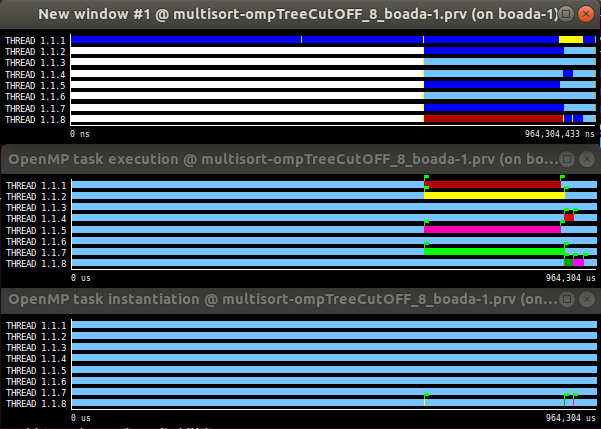
\includegraphics[scale=0.75]{images/paraverTreeCutoffNoZoom.PNG}
    \caption{Paraver with a Tree - cutoff strategy}
    \label{paravercutoff}
\end{figure}
In Figure \ref{paravercutoff}, at the bottom, we can see how very few tasks are created. In fact, by looking at the middle graphic which shows task execution, we can appreciate how 4 long sorting tasks are executed and, after, 2 merges and another final merge at the end. This shows perfectly what happens at a given recursion level: the list is divided into 4 parts, each of this is sorted, then we group them into pairs, merge each pair, and finally we take the resultant 2 parts and merge them into one list of the original size.

\medskip
\begin{figure}[H]
    \centering
    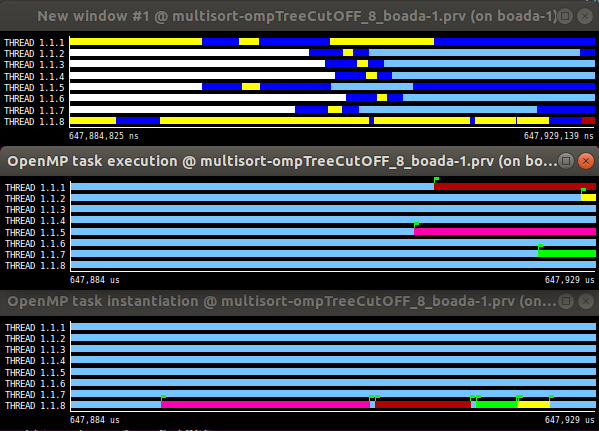
\includegraphics[scale=0.75]{images/paraverTreeCutoffZoom.PNG}
    \caption{Paraver with a Tree - cutoff strategy, zoomed in}
    \label{paravercutoffZoom}
\end{figure}

Figure \ref{paravertreeZoom} doesn't give us much insight this time, as with no zoom it was very easy to see what was happening.
\\
Now the question arises of which cutoff value will bring the best results in terms of execution time. We know that a too-small cutoff will make the program almost sequential, losing the benefits of parallelization; but a too-big cutoff will bring back the big task-creation overhead of the normal tree strategy. The sweet spot where we can tip off all the benefits should fall somewhere in the middle. In fact, we are given a script called \textit{submit-cutoff.sh} which the execution time for each cutoff value with fixed parameters. Unfortunately, we cannot display the plot generated as we are given an error of "cutoff-omp.jgr,18: Reading Points, no y value for x=1.747622". We could, nonetheless, read the txt file created, so we parsed the execution times and created the following plot shown in Figure \ref{cutoffvalue}.
\medskip
\begin{figure}[H]
    \centering
    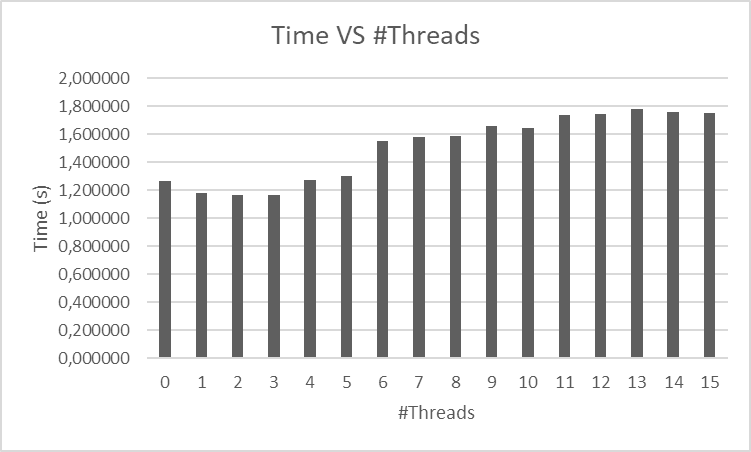
\includegraphics[scale=0.6]{images/bestCutoff.png}
    \caption{Execution time for different cutoff values}
    \label{cutoffvalue}
\end{figure}
\\
Here it's easy to see that the shortest execution times are for cutoff values 2 and 3. More precisely, 2 is slightly better, so this is the value we will use to analyze the strong scalability of this strategy.
\\
\medskip
\begin{figure}[H]
    \centering
    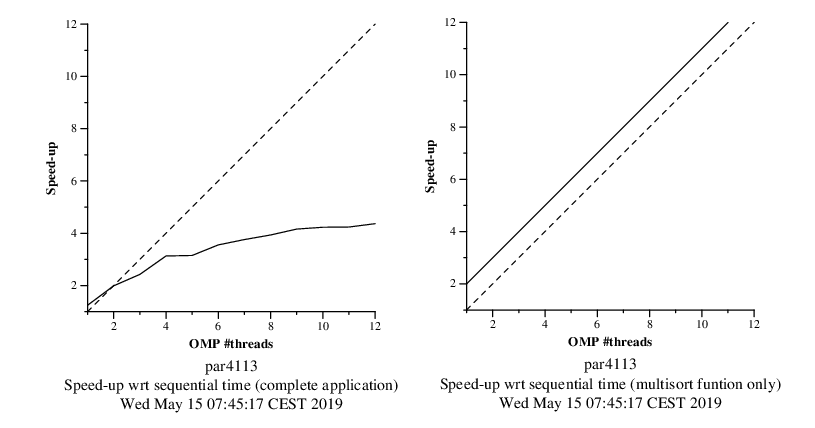
\includegraphics[scale=0.75]{images/cutoffStrong.png}
    \caption{Speed-up with a Tree - cutoff strategy}
    \label{speedupcutoff}
\end{figure}
\\
Looking at the strong scalability plots with a cutoff value of 2 in Figure \ref{speedupcutoff}, it appears that the more threads, the better again, which is good, as we can take advantage of all the threads used (it does, however, follow a logarithmic increase, which doesn't get much better for big values). This time, however, the maximum speedup we achieve surpasses 4, which is the best we have seen yet. What's more, if only looking at multisort functions, we achieve an ideal speedup which keeps increasing linearly with the number of threads. This means our hypothesis was true, adding a cutoff greatly improves scalability and, therefore, execution times.

\subsection{Optional 1}
We executed the scalability script with the tree strategy again with each different kind of Boada node: execution, cuda and execution2. For each one, we used a different max number of threads, according to their specifications.
\begin{itemize}
    \item execution: 2 sockets/node * 6 cores per socket * 2 threads per core = 24 threads
    \item cuda: 2 sockets/node * 6 cores per socket * 2 threads per core = 24 threads
    \item execution2: 2 sockets/node * 8 cores per socket * 1 thread per core = 16 threads
\end{itemize}
These are the max threads we used for each node, and the results are the following, shown in Figure \ref{executionstrong}, \ref{cudastrong} and \ref{execution2strong}.
\\
\medskip
\begin{figure}[H]
    \centering
    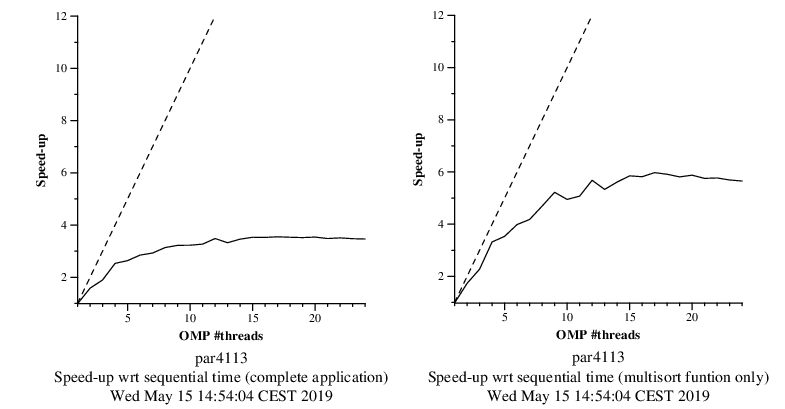
\includegraphics[scale=0.75]{images/executionStrong.png}
    \caption{execution scalability plot}
    \label{executionstrong}
\end{figure}
\\
\medskip
\begin{figure}[H]
    \centering
    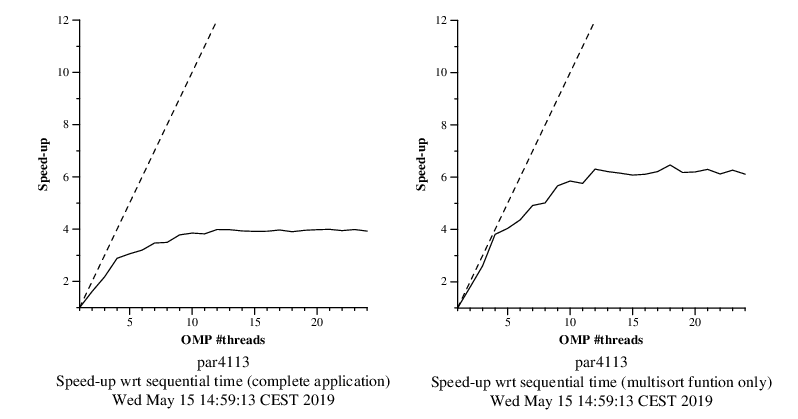
\includegraphics[scale=0.75]{images/cudaStrong.png}
    \caption{cuda scalability plot}
    \label{executionstrong}
\end{figure}
\\
\medskip
\begin{figure}[H]
    \centering
    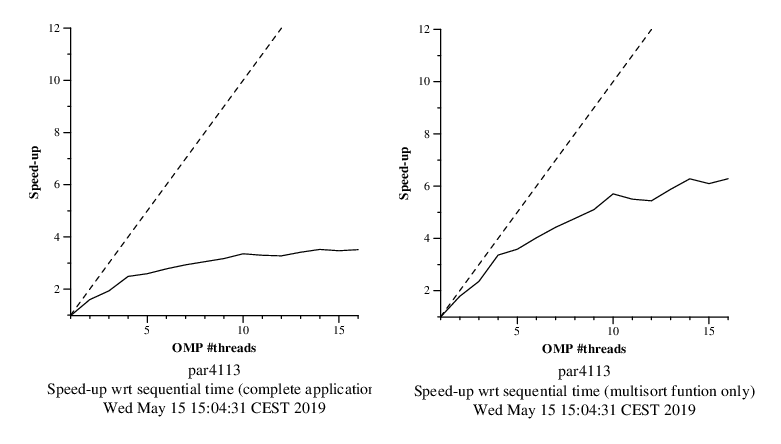
\includegraphics[scale=0.75]{images/execution2Strong.png}
    \caption{execution2 scalability plot}
    \label{executionstrong}
\end{figure}
\\
As seen, from 16 threads and up, speed-up gets stuck and actually starts to decrease by a small amount, due to the added overhead of initializing and synchronizing so many threads. This isn't a problem with execution2, as it has exactly this number of threads, but for other node kinds it means not being able to take full advantage of their processor.

\subsection{Optional 2}
In this section we are asked to parallelize the initialization of \textit{data} and \textit{tmp} vectors in the tree strategy multisort. Since they are initialized in a for loop which goes through all the positions to set them to some value, we just need to parallelize these 2 for loops (q for each vector) in their respective initialization functions, adding a \textit{#pragma omp parallel for} call:
\begin{lstlisting}[frame=single]
static void initialize(long length, T data[length]) {
   long i;
   #pragma omp parallel for
   for (i = 0; i < length; i++) {
      if (i==0) {
         data[i] = rand();
      } else {
         data[i] = ((data[i-1]+1) * i * 104723L) % N;
      }   
   }   
}

static void clear(long length, T data[length]) {
   long i;
   #pragma omp parallel for
   for (i = 0; i < length; i++) {
      data[i] = 0;
   }   
}
\end{lstlisting}
Now for initialize(), this might arise some concern as in case the position i hasn't a value 0, it will fill it with a modified value of the previous position, which because of the parallelization, might not have yet been initialized. This is not really a problem here as in C, an unset memory position assumes some value (usually zero but not granted), and therefore there are no errors during execution (since we want random values, we don't care wither for what value C gets from unset positions as long as it's a number).
\\
When doing this, we obtain the following scalability plot seen in Figure \ref{fullParStrong}.
\\
\medskip
\begin{figure}[H]
    \centering
    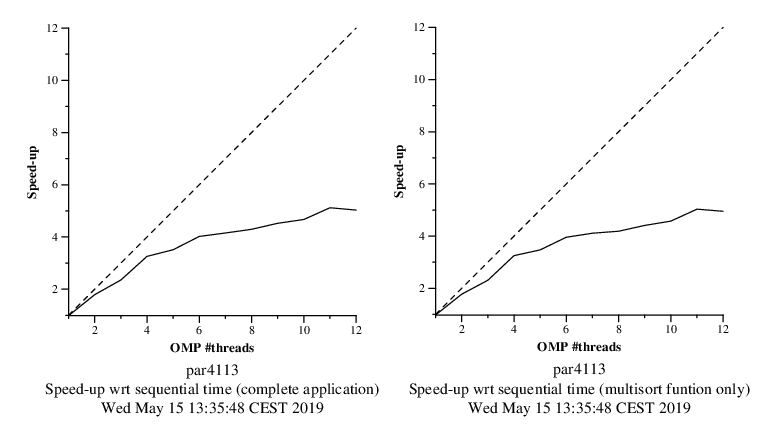
\includegraphics[scale=0.75]{images/fullParStrong.png}
    \caption{Full parallelization scalability plot}
    \label{fullParStrong}
\end{figure}
\\
As observed, the scalability plot for multisort function only is very similar to the one we got whithout parallelizing the initialization of the vectors. However, there has been a big improvement in the overall scalability of the program, and this is due to a big part of the execution time of the non-multisort functions being taken by the initialization of the vectors. When parallelized, this initial section is much faster, and because of the big size of the vectors, it actually benefits more and more the more threads it has. It is a big improvement over the non-parallelized initialization. Following, we can see the traces generated in Figure \ref{paraverfull}. We used the \textit{Parallel Functions Duration} configuration (2nd starting from the top) in addition to the tasks ones because we are not creating tasks for the initialization of the vectors (because we are using #pragma omp for), and so these will not show as tasks. 
\\
\medskip
\begin{figure}[H]
    \centering
    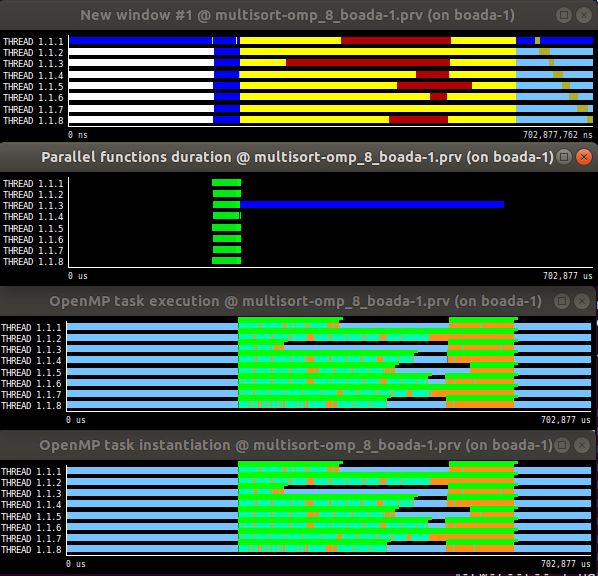
\includegraphics[scale=0.75]{images/paraverFull.PNG}
    \caption{Full parallelization Paraver traces}
    \label{paraverfull}
\end{figure}
\\
It's easy to see that all 8 threads contribute to the initialization of the 2 vectors before starting the sorting tasks. Since we didn't use \textit{taskloop} and instead used \textit{for}, this is interpreted as parallel functions (hence the extra configuration to visualize it).

\section{Parallelization and performance analysis with dependent tasks}
To execute our code using dependent tasks, we used \textbf{#pragma omp task depend (out:)} and \textbf{#pragma omp task depend (in:)}.
\\
Inside the multisort function, for each multisort call, we declare a \textbf{#pragma omp task depend (out:)} with different outs, then on the next two merge functions, they wait until two specific multisort functions end, and finally another merge that waits for the last two merge functions. This way we achieve a tree strategy avoiding small merging tasks to wait for parts of the list they do not need being sorted. 
\medskip

\begin{lstlisting}[frame=single]
void merge(long n, T left[n], T right[n], T result[n*2], long start, long length){
    if (length < MIN_MERGE_SIZE*2L) {
        // Base case
        basicmerge(n,left,right,result,start,length);
    } else {
        //Recursive decomposition
        #pragma omp task
        merge(n,left,right,result,start,length/2);
        #pragma omp task
        merge(n,left,right,result,start+length/2,length/2);
        #pragma omp taskwait
    }
}

void multisort(long n, T data[n], T tmp[n]){
    if(n>= MIN_SORT_SIZE*4L){
        #pragma omp task depend(out:data[0])
        multisort(n/4L,&data[0],&tmp[0]);
        #pragma omp task depend(out:data[n/4L])
        multisort(n/4L,&data[n/4L],&tmp[n/4L]);
        #pragma omp task depend(out: data[n/2L])
        multisort(n/4L, &data[n/2L], &tmp[n/2L]);
        #pragma omp task depend(out: data[3L*n/4L])
        multisort(n/4L, &data[3L*n/4L], &tmp[3L*n/4L]);
        #pragma omp task depend(in: data[0], data[n/4L]) depend(out: tmp[0])
        merge(n/4L, &data[0], &data[n/4L], &tmp[0], 0, n/2L);
        #pragma omp task depend(in: data[n/2L], data[3L*n/4L]) depend(out:tmp[n/2L])
        merge(n/4L, &data[n/2L], &data[3L*n/4L], &tmp[n/2L], 0, n/2L);
        #pragma omp task depend(in: tmp[0], tmp[n/2L])
        merge(n/2L, &tmp[0], &tmp[n/2L], &data[0], 0, n);
        #pragma omp taskwait
    } else {
        //Base case
        basicsort(n,data);
    }
}

int main(...) {
    ...
    #pragma omp parallel
    #pragma omp single
    multisort(N, data, tmp);
    ...
}
\end{lstlisting}
\\
Figure \ref{paraverdepend} shows the Paraver traces generated when executing this version of multisort.
\\
\medskip
\begin{figure}[H]
    \centering
    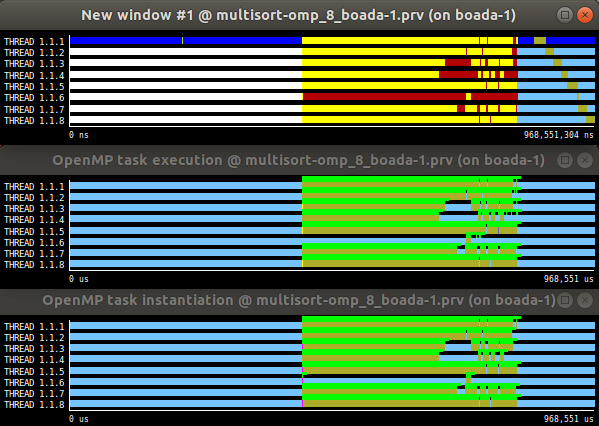
\includegraphics[scale=0.75]{images/paraverDependNoZoom.PNG}
    \caption{Paraver traces specifying individual dependencies}
    \label{paraverdepend}
\end{figure}
\\
As seen, traces in Figure \ref{paraverdepend} are very similar to the ones we got with the tree strategy in Session 2 (Figure \ref{paravertree}). We know, however, that this time merge tasks do not have to wait for the 4 previous sorts to end in order to start merging. Since dependencies are now individually specified, the task merging part 1/4 and 2/4 will start as soon the sorting of those two parts has finished and there are threads available. With the tree strategy in Session 2 this didn't happen, both merges had to wait for the 4 parts of the list to be sorted. The final merge, however, still has to wait for both merges to be complete, and since both are the same size, we don't think starting one earlier and waiting for the last one will make a significant improvement when compared to starting both at the same time in parallel. We will check whether this is true or not by looking at the scalability plot in Figure \ref{strongdepend}.
\\
\medskip
\begin{figure}[H]
    \centering
    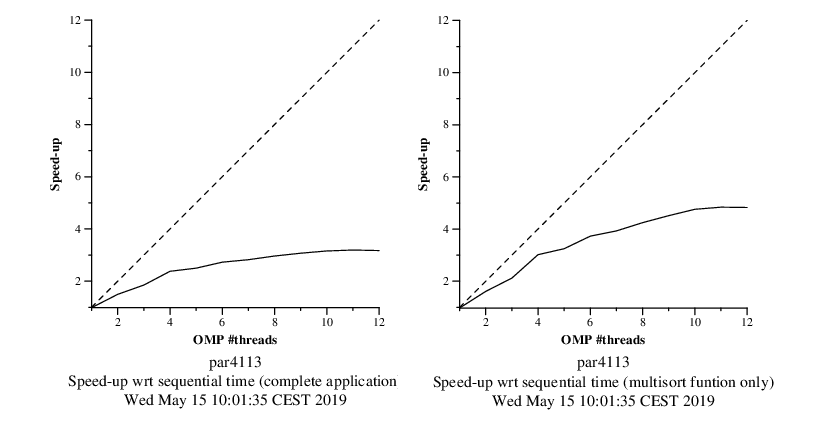
\includegraphics[scale=0.75]{images/dependStrong.PNG}
    \caption{Strong scalability plot specifying individual dependencies}
    \label{strongdepend}
\end{figure}
\\
As thought, the scalability plot shows that we can achieve a similar speedup as the one we got when using tree strategy without setting individual dependencies. It benefits of having many threads for the same reason explained in the tree strategy section, increases logarithmically and has what looks like an asymptotic limit at around a speedup of 3.5 . The speedup looking only at the multisort functions is also pretty similar to the tree strategy of Session 2. As said earlier, we think this is due to the final merge which merges the result of the 2 smaller merges still has to wait for both to finish and so improvement isn't much.

\section{Conclusions}

The main goal of this laboratory session was to study different strategies to parallelize the multisort algorithm. After seeing these different methods, we can conclude, as shown in the report, that the Tree strategy is more effective than the Leaf strategy in terms of parallelization, and it gets even better when using a cutoff at depth 2 to reduce the amount of tasks generated. Also, explicitly declaring individual dependencies for each task results in a marginally better improvement because is capped due to big merges depending on having all parts of the list sorted. If we wanted to take more advantage of parallelization, we should parallelize the initialization of the vectors as done in the 2nd optional section.

\end{document}